\documentclass[conference]{IEEEtran}
\usepackage{times}

\ifCLASSINFOpdf
  \usepackage[pdftex]{graphicx}
  \graphicspath{images/}
\else
  \usepackage[dvips]{graphicx}
  \graphicspath{images/}
\fi

% numbers option provides compact numerical references in the text.
\usepackage[numbers]{natbib}
\usepackage{multicol}
\usepackage[bookmarks=true]{hyperref}
\usepackage{color}
\usepackage{amsmath}
\usepackage{amsfonts}

\usepackage{algorithmic, algorithm}

\usepackage[squaren, Gray, cdot]{SIunits}

% Commands and other stuff
\DeclareMathOperator*{\argmin}{arg\,min}
\newcommand{\PFA}[1]{{\color{red}\fbox{PFA:} #1}}
\newcommand{\TM}[1]{{\color{blue}\fbox{TM:} #1}}
\newcommand{\OS}[1]{{\color{green}\fbox{OS:} #1}}

\begin{document}

\title{Reliable Indoor Navigation on Humanoid Robots using
  Vision-Based Localization}

% You will get a Paper-ID when submitting a pdf file to the conference system
\author{Author Names Omitted for Anonymous Review. Paper-ID [add your ID here]}

%\author{\authorblockN{Michael Shell}
%\authorblockA{School of Electrical and\\Computer Engineering\\
%Georgia Institute of Technology\\
%Atlanta, Georgia 30332--0250\\
%Email: mshell@ece.gatech.edu}
%\and
%\authorblockN{Homer Simpson}
%\authorblockA{Twentieth Century Fox\\
%Springfield, USA\\
%Email: homer@thesimpsons.com}
%\and
%\authorblockN{James Kirk\\ and Montgomery Scott}
%\authorblockA{Starfleet Academy\\
%San Francisco, California 96678-2391\\
%Telephone: (800) 555--1212\\
%Fax: (888) 555--1212}}


% avoiding spaces at the end of the author lines is not a problem with
% conference papers because we don't use \thanks or \IEEEmembership


% for over three affiliations, or if they all won't fit within the width
% of the page, use this alternative format:
%
%\author{\authorblockN{Michael Shell\authorrefmark{1},
%Homer Simpson\authorrefmark{2},
%James Kirk\authorrefmark{3},
%Montgomery Scott\authorrefmark{3} and
%Eldon Tyrell\authorrefmark{4}}
%\authorblockA{\authorrefmark{1}School of Electrical and Computer Engineering\\
%Georgia Institute of Technology,
%Atlanta, Georgia 30332--0250\\ Email: mshell@ece.gatech.edu}
%\authorblockA{\authorrefmark{2}Twentieth Century Fox, Springfield, USA\\
%Email: homer@thesimpsons.com}
%\authorblockA{\authorrefmark{3}Starfleet Academy, San Francisco, California 96678-2391\\
%Telephone: (800) 555--1212, Fax: (888) 555--1212}
%\authorblockA{\authorrefmark{4}Tyrell Inc., 123 Replicant Street, Los Angeles, California 90210--4321}}

% LAAS authors:
%\author{ \parbox{3 in}{\centering Thomas Moulard, Florent Lamiraux, Olivier Stasse\\
%    LAAS-CNRS, Universit\'e de Toulouse\\
%    7, avenue du Colonel Roche\\
%    31077 Toulouse cedex 4, France\\
%    {\tt\small thomas.moulard@laas.fr}}
%}

\maketitle

\begin{abstract}
Reliable localization on a humanoid robot is a \textit{sine qua non} condition to succeed in realizing complex robotics scenarios. Before dealing with perturbations and online modification of the environment, one has to make sure that the planned trajectory alone will be correctly followed. This paper demonstrates that a control framework suited to humanoid robots relying on a vision-based localization system can achieve this goal. Our localization framework is based on a real-time vision-based localization system that assumes that a pre-existing 3D map of the environment exists and allows to obtain accurate results in complex robotics scenarios. By compensating for execution errors such as drifts and robot model errors, the HRP-2 robot is able to achieve high precision tasks. 
\end{abstract}

\begin{IEEEkeywords}
  Humanoid robots, Localization, Motion Planning, Robot Control, Stereo Vision
\end{IEEEkeywords}

\IEEEpeerreviewmaketitle

\section{Introduction}~\label{sec:introduction}

In this paper, we consider the problem of real-time reliable
trajectory execution for humanoid robots. A precise localization on a
humanoid robot is both crucial to achieve reliable trajectory
execution and challenging due to humanoid robots specific features. We
propose a novel control architecture for humanoid robots where the
current localization is used by the robot controller and planner
trajectory. The objective of this work is to localize the humanoid
robot HRP-2~\cite{Kaneko04icra} while it is navigating through an
indoor environment.

Localization is crucial on a humanoid robot as its position cannot be
controlled directly. Legs motion are planned under the assumption that
all contacts will be perfect (i.e.\ no friction) during the
movement. This is not the case in practice and leads to execution
errors which cannot be ignored. Moreover, reactive control algorithms
rely on simplified dynamics models such as the \textit{Linear Inverted
  Pendulum} model~\cite{Kajita01iros}. These imply a gap between the
generated motion and the executed one. Therefore, localization is
necessary to ensure a consistent robot behavior.
\TM{Highlight the fact that the planner uses the whole body dynamics
  whereas the correction uses the LIP}

However, localization on a humanoid robot is challenging. Mobile
robots odometry can be computed using wheel encoders and give a
reasonable hint on the current robot motion. 2D maps can also be used
to simplify the navigation through indoor environments. This is not
the case on a legged robot on which 3D localization is required and
where no encoder based reliable odometry exists.
%
\begin{figure}[ht]
  \begin{center}
    \includegraphics[width=.9\linewidth]{images/demo1.jpg}
  \end{center}
  \caption{HRP-2 dropping a ball on a shelf after having navigated through an indoor environment. Navigation followed by manipulation are typical scenarios where walking drift can prevent a task from being accomplished.\label{fig:xp_final}}
\end{figure}
%
All these reasons make localization a cornerstone of reliable
trajectory execution on humanoid robots. To obtain an accurate
localization of the robot in the environment, we employ fast
vision-based localization techniques~\cite{Alcantarilla10icra} that
assume that a prior 3D map of the environment exists. By means of
\textit{visibility prediction}~\cite{Alcantarilla11icra}, a fast and
robust data association between a large map of 3D points and perceived
2D features in the image can be performed very efficiently. Firstly,
the 3D map of the environment is computed by using visual Simultaneous
Localization and Mapping~(SLAM)~\cite{Davison07pami,Konolige08tro}
techniques.

In this article, the past results in vision processing on humanoids
robots are presented in
Section~\ref{sec:related}. Section~\ref{sec:architecture} details how
the vision is linked to the robot controller via our proposed control
scheme. The vision-based localization algorithm is described in detail
in Section~\ref{sec:vision}. The experimental results are discussed
and compared to motion capture data in
Section~\ref{sec:results}. Finally, conclusions and future work are
described in Section~\ref{sec:conclusions}.

%%% Local Variables:
%%% ispell-local-dictionary: "american"
%%% LocalWords:  odometry HRP roadmap
%%% End:

\section{Related Work}\label{sec:related}
Cameras seem to be an appealing sensor for humanoid robotics applications: they are small, cheap and light-weight
compared to other sensors such as laser scanners. Despite of this, there have been only limited attempts at vision-based
localization for humanoid robots. Ozawa et al.~\cite{Ozawa05smc} proposed to use stereo visual odometry to create local 3D maps for
online footstep planning. The main drawback of this approach is the drift created by the accumulation of errors that typically
occur in visual odometry systems~\cite{Kaess09icra}. 

Other past experiments where vision algorithms have been used to construct navigation maps for humanoid robots are~\cite{Michel05humanoids,Michel06icra}. However, most of these works were focused on the humanoid trajectory generation replanning problem. In this paper, our approach is different: the objective is to execute a planned trajectory without any online replanning. The computation of a whole-body trajectory remains very costly and do not meet the real-time requirements of small robots such
as Nao~\footnote{http://www.aldebaran-robotics.com/en/}. Therefore, local trajectory deformation is important to achieve high reactivity and to avoid unnecessary computations.

The work by Dune et al.~\cite{Dune10iros} relies on visual servoing to compute a center of mass reference velocity to control the walking trajectory generation algorithm described in~\cite{Herdt10adr}. By
computing the foot placement online, one can control directly the robot center of mass velocity on a 2D plane and get rid of most of the complexity of the walking process. This approach is extremely interesting, but unfortunately does not take into account obstacles in the environment. Also, this algorithm is not suited for trajectory tracking which is our objective. The following works~\cite{Harada04humanoids,Morisawa07icra} aim at allowing sudden changes in the robot trajectory. Again, the objectives pursued by these works and our work differ as they alter the initial plan to react to changes in the environment.

~\citet{Davison07pami} showed successful monocular SLAM results for small indoor environments using the HRP-2 robot. This approach, known as \textit{MonoSLAM}, is a monocular Extended Kalman Filter (EKF) vision-based system, that allows building a small map of sparse 3D points. However, acceptable results were only obtained when the pattern generator, the robot odometry and inertial sensing were fused to aid
the visual mapping into the EKF framework as it was shown in~\cite{Stasse06iros}. The fusion of the information from different sensors can reduce considerably the uncertainty in the camera pose and the 3D map points involved in the EKF process, yielding better localization and mapping results.

Despite of this, EKF-based approaches have important drawbacks such as the limited number of 3D points that can be
tracked and divergence from the true solution due to linearization errors. As shown in~\cite{Strasdat10icra}, nonlinear
optimization techniques such as bundle adjustment~\cite{Mouragnon09ivc} are superior in terms of accuracy to filtering based methods, and
allow tracking many hundreds of features between frames. In this paper we use the framework described in~\cite{Alcantarilla12auro}, where a stereo visual SLAM algorithm based on local bundle adjustment is used to compute a 3D map of the robot's environment. Then, we use the prior 3D map for an efficient data association obtaining a real-time accurate localization of the robot within the 3D environment.

%%% Local Variables:
%%% ispell-local-dictionary: "american"
%%% LocalWords:  odometry HRP servoing replanning Nao MonoSLAM Kalman EKF al
%%% LocalWords:  Ozawa linearization
%%% End:

\section{Robotics Framework for Reliable Trajectory Execution}\label{sec:architecture}

\subsection{Robotics Architecture}

In this section the main components of our robotics framework for
reliable trajectory estimation will be described. The HRP-2 robot
embeds two computers. One is dedicated to motor control and the other
one to vision processing. Fig.~\ref{fig:framework_overview}
illustrates the complete robotics distributed infrastructure used in
this experiment. It relies heavily on both OpenHRP and ROS to
integration the different modules altogether.
%
\begin{figure}[ht!]
  \begin{center}
    \includegraphics[width=\linewidth]{images/rss_framework.png}
  \end{center}
  \caption{Complete robotics framework overview. Let
    $\mathbf{I}_{\text{left}}$, $\mathbf{I}_{\text{right}}$ be
    respectively the left and right camera
    images. $\mathit{T}_{\text{cam}}$, $\mathit{\hat{T}}_{\text{cam}}$
    respectively the planned and estimated camera
    position. $\mathbf{\gamma}$ the concatenation of the left ankle,
    right ankle, upper body and center of mass
    trajectories. $\mathbf{\gamma'}$ the trajectories reshaped by
    taking into account execution
    errors.\label{fig:framework_overview}}
\end{figure}
% The control is based on a task based
controller~\cite{Mansard09icar}. A task is a function which associates
\mbox{$\mathbf{q} \in \mathcal{C}$} the robot configuration to
\mbox{$e(\mathbf{q}) \in \mathbb{R}$} an error. The controller embeds
a solver which is able to generate a control law which minimizes the
error for a given stack of tasks.

\begin{enumerate}
\item Using a given stack of tasks, this controller computes the joint
  velocities $\mathbf{\dot{q}}$ which realizes the tasks. Our stack of
  tasks ensures that the left ankle, right ankle, center of mass and
  upper level posture reference positions are followed. The reference
  trajectories are computed off-line by the planner described in
  \cite{Dalibard11humanoids}.
\item The reference trajectories can be post-processed by the
  controller to reshape them on the fly. The controller has been
  extended to incorporate a module which can, given an execution error
  estimation, cancel them automatically by changing the future robot
  trajectory.
\item This estimation of the execution error is computed on the
  computer dedicated to vision. By comparing the planned left ankle
  trajectory and the estimated one, it is possible to compute an
  estimation of the execution error.
\item The planned left ankle position is computed using both the
  camera position and the relative transformation from the camera to
  the left ankle. This transformation can be deduced from the robot
  configuration and its model using forward kinematics.
\end{enumerate}

\subsection{Closed-loop tracking}

Closed-loop trajectory tracking consists in following a precomputed
trajectory while compensating for execution errors. Systems are often
composed of four components:
\begin{enumerate}
\item a trajectory generator component,
\item a localization component providing an estimation of the robot
  position,
\item an error estimation component computing the error between the
  planned position and the localization of the robot,
\item and a component reshaping the planned trajectory to compensate
  for the above error.
\end{enumerate}


The trajectory generator provides two reference data: the footstep
sequence, a set of footsteps $S_i$ such as \mbox{$0 \leq i \leq
  n^{\text{step}}$} and a whole-body trajectory \mbox{$\gamma(t \in
  [t_{\text{min}}, t_{\text{max}}]) \in \mathcal{C}$}. One advantage
of the proposed control scheme is to alter the future footstep
positions to avoid singularities. Given a known perturbation of the
footstep sequence, it is then possible to deduce the correction that
should be applied to the feet and center of mass trajectories. Once
those trajectories are computed, inverse geometry can be used to
regenerate the joints trajectories.


One iteration of the control loop is described by
Algorithm~\ref{fig:control_loop} and can be summarized as:
\begin{enumerate}
\item estimate the robot position,
\item compute the position error \mbox{$\delta \mathbf{x}$},
\item filter the error to avoid perturbing too much the initial
  trajectory and to absorb localization noise,
\item recompute the next steps positions to compensate execution
  errors and make sure the feet will land on the planned position,
\item check if the recomputed next step is feasible,
\item regenerate smooth trajectories for the feet, center of mass and
  ZMP.
\item regenerate the joints trajectories. This step is denoted by
  \mbox{$\gamma \bigoplus \delta \gamma$} in the algorithm. The
  \mbox{$\gamma \bigoplus \delta \gamma$} operation returns $\gamma$
  altered by the rigid transformation \mbox{$\delta \gamma$}. $\delta
  \gamma$ is the perturbation applied to the whole-body trajectory and
  is not directly computed as the inverse geometry is directly applied
  on the updated body positions.
\end{enumerate}


\begin{algorithm}
  \begin{algorithmic}
    \REQUIRE {$\gamma$, $t_{\text{current}}, t_{\text{next\_correction}}$}
    \ENSURE {$\gamma$, $t_{\text{current}}, t_{\text{next\_correction}}$}
    \IF {$\gamma(t_{\text{current}})$ is double support \AND
      $t_{\text{current}} \geq t_{\text{next\_correction}}$}
    \STATE estimate robot position $\mathbf{\hat{x}}$
    \STATE compute robot position error $\delta \mathbf{x}$
    \STATE compute offset $\delta \gamma$ absorbing the execution
    error $\delta \mathbf{x}$
    \IF {the perturbation $\delta \gamma$ can be applied}
    \STATE $\forall t \in [t_{\text{current}}, t_{\text{max}}],
    \gamma(t) \leftarrow \gamma(t) \bigoplus \delta \gamma(t)$
    \STATE $t_{\text{next\_correction}} \leftarrow t_{\text{current}} + 2 T_{\text{step}}$
    \ENDIF
    \ENDIF
    \STATE $\mathbf{q} \leftarrow \gamma(t_{\text{current}})$
    \STATE $t_{\text{current}} \leftarrow t_{\text{current}} + \Delta t$
  \end{algorithmic}
  \caption{Control loop at time $t_{\text{current}}$ achieving a
    closed-loop following of trajectory $\gamma$ (next correction will
    be applied at
    $t_{\text{next\_correction}}$). \label{fig:control_loop}}
\end{algorithm}


First, the robot position $\hat{\mathbf{x}}$ is perceived. The
localization system will not be detailed in this paper, see
\cite{08ijhr.stasse, 06humanoids.thompson} for instance for more
details. Although common limitations of these systems are taken into
account. The precision of the robot estimation does not decrease over
time, but can vary during the execution. This produces a noise which
may perturb the control scheme. The localization system can also fail
to provide an estimation or even sometimes provide aberrant values.

Secondly, an error $\mathbf{\delta \mathbf{x}}$ is computed by
comparing the planned and estimated position of the tracked reference
body. A threshold is applied to this value to bound the applied
corrections. In practice, it also filters out outliers and the noise
that the localization system may introduce in the system.

Then, the relative position of the next footstep w.r.t. to the current
one is changed to compensate the perceived
error. Fig.~\ref{fig:footstepreplan} illustrates this process.


From this point, smooth trajectories can be regenerated for feet and
center of mass. To ensure smoothness, the trajectory correction is
progressively applied during the next two steps. To finish, joint
values are recomputed using these new reference trajectories.



Additionally, a test is added to check that a correction can be
computed for the current time $t_{\text{current}}$. A correction can
be applied if no correction is being applied,
i.e.\ \mbox{$t_{\text{current}} \geq t_{\text{next\_correction}}$} and if the
robot is in the double support phase. Indeed starting a correction in
the middle of a step would be dangerous and starting a correction
while another correction is being applied would lead to erroneous
results.


Previous works such as \cite{04humanoids.harada, 07icra.morisawa} aim
at allowing sudden changes in the robot trajectory. The proposed
control scheme is different and aim at following as closely as
possible a preplanned trajectory.


\paragraph{Estimation of the position error}

We make the assumption that an external system provides
\mbox{$\hat{\mathbf{x}} \in \text{SE}(2)$}, an estimation of the
current robot position.

If $\mathbf{x} \in \text{SE}(2)$ is the robot planned position and
$\hat{\mathbf{x}} \in \text{SE}(2)$ the robot localization, the
position error is defined by:

\begin{equation} \label{eq:errorpos}
  \mathbf{\delta x} = \mathbf{x} . \hat{\mathbf{x}}^{-1}
\end{equation}

In Eq. (\ref{eq:errorpos}), $\mathbf{\delta x}(t)$ can be
interpreted as the planned robot position with respect to the current
robot position at time $t$. By consequence, at the beginning of the
trajectory $t_{\text{min}}$, the error is always equal to zero:

\begin{equation} \label{eq:errorpos_prop}
  \delta \mathbf{x}(t_{\text{min}}) = 0
\end{equation}

\paragraph{Footstep sequence modification}


Given a position error of the waist, it is possible to alter the
remaining steps in the footstep sequence to absorb this offset.

The purpose of this step is to take into consideration that the
previous step has not been executed correctly, leading to a different
relative position than the one which has been initially planned. To
cancel the error, the next footsteps positions will be modified
so that the robot will step in the planned locations.


The footstep positions are \mbox{$S \in
  \text{SE}(2)^{n^\text{step}}$}. Let consider $\mathbf{\delta {x}}$,
the current position error, \mbox{$S^{\text{future}} \subset S$} the
steps which have not been played yet. The footstep positions will be
changed according to the following computation:

\begin{equation} \label{eq:footstepmodif}
  \forall s \in S^{\text{future}}, s \gets \mathbf{\delta {x}} . s
\end{equation}


\paragraph{Whole-body trajectories modification}

A new placement of the next feet has been computed. It is now necessary
to modify the two feet and the center of mass trajectories
synchronously to reach the corrected foot prints.

The correction is computed by considering the simplified model
introduced in section \ref{problem}. Hence, no hypothesis is done on
the strategy used to plan the reference trajectories. One interest of
this approach is to totally dissociate the planning and correction
algorithms. To compute a small perturbation the simplified model is
sufficient. It allows extremely reactive correction without
compromising the overall trajectory quality.


The linearized inverse pendulum model allows the computation of the
center of mass trajectory $\mathbf{c}(t)$ given a ZMP trajectory
$\mathbf{z}(t)$ by solving Eq.~(\ref{eq:zmp1}). Considering $\mathbf{r}$ a
polynomial depending only of $\mathbf{z}$, $(V_x, V_y, W_x, W_y)$ free
parameters used to constrain the initial position and velocity of the
center of mass, a general following form of a polynomial center of
mass trajectory is:

\begin{equation} \label{eq:zmpsol}
  \mathbf{c}(t) = \cosh(\sqrt{\frac{g}{z_c}}.t) . \mathbf{V} + \sinh(\sqrt{\frac{g}{z_c}}.t) . \mathbf{W} + \mathbf{r}(t)
\end{equation}

Given the formulation in Eq.~(\ref{eq:zmpsol}), it is possible to
continuously modify the center of mass trajectory to make it follow
\mbox{$\bar{\mathbf{z}}(t)$} the corrected trajectory. This new
trajectory can be expressed as the sum of two polynomials:

\begin{equation} \label{eq:zmpsolcor}
  \bar{\mathbf{c}}(t) = \cosh(\sqrt{\frac{g}{z_c}}.t) . \mathbf{V} +
  \sinh(\sqrt{\frac{g}{z_c}}.t) . \mathbf{W} + \mathbf{r}(t) + \mathbf{\Delta}(t)
\end{equation}

To apply smoothly the correction from $t_1$ to $t_2$, several
constraints expressed in Eq.~\ref{eq:cst} have to be respected.
$\delta \mathbf{x}_x$ and $\delta \mathbf{x}_y$ are respectively the
$x$ and $y$ components of the 2d rigid transformation $\delta
\mathbf{x}$.

\begin{equation}
\begin{aligned}
  \mathbf{\Delta}(t_1) &= 0\\
  \mathbf{\Delta}(t_2) &= \left(
  \begin{array}{c}
    \delta \mathbf{x}_x \\
    \delta \mathbf{x}_y
  \end{array}
  \right)\\
  \frac{\partial \mathbf{\Delta}}{\partial t}(t_1) = \frac{\partial
    \mathbf{\Delta}}{\partial t}(t_2) &= 0
\end{aligned}
\label{eq:cst}
\end{equation}

These four constraints determine the polynomial four parameters
leading to the curve illustrated by Fig.~\ref{fig:transition}.


This reshapes the center of mass trajectory by taking advantage of the
linear formulation of the simplified model. Additionally, the feet
trajectories are modified to reach the corrected positions at the end
of the step. The smooth correction is also obtained by using a third
degree polynomial with similar constraints: initial position remains
as before, the goal position must fit the corrected position and the
velocity of the correction is equal to zero at the beginning and the
end of the transition. Fig.~\ref{fig:traj} compares resulting
trajectories before and after the correction.


These three corrections must be executed in the correct order: as
stated before a correction is computed during a double support phase
and applied during the next two steps. We will make the assumption,
without any loss of generality, that the next flying foot is the left
one. In that case the correction of the left foot is progressively
applied during the single support phase. During the ZMP shift of this
step, the center of mass correction is also applied. Then, during the
next step, the correction of the right foot is applied. The timeline
of the correction is illustrated by Fig.~\ref{fig:traj}.


\PFA{This section can be dedicated to the control and planning framework}

%%% Local Variables:
%%% ispell-local-dictionary: "american"
%%% LocalWords:  odometry HRP
%%% End:


\section{Vision Processing}\label{sec:vision}
Our computer vision module comprises two different stages: first, a stereo visual SLAM module for building a persistent 3D map of the environment and second a vision-based localization framework with visibility prediction that assumes that a prior 3D map of the environment is given. Prior to any SLAM or localization processing, we correct the distortion of the images and perform stereo rectification. Stereo rectification simplifies considerably the stereo correspondences problem and disparity maps can be easily obtained with the rectified images. More details of the visual SLAM and vision-based localization algorithms can be found in~\cite{Alcantarilla12auro}. In this section, we will briefly describe the main components of our localization framework assuming that we already have a prior 3D map of the environment. Given a prior 3D map of the environment we can use the computed map for fast and robust localization. In this context we employ the visibility prediction technique described in~\cite{Alcantarilla11icra,Alcantarilla12auro} to perform an efficient data association between known 3D points and detected 2D features.

Our localization framework is composed of two different modules: initialization and a combination of vision-based
localization with visibility prediction and stereo visual odometry.

\subsection{Initialization and Re-Localization}
At this stage, the robot is lost and can be located in any area of the map. Therefore, we need to find an initial camera pose to start the
vision-based localization algorithm. For this purpose we detect 2D features in the new image using the Harris corner detector~\cite{Harris88avc} at different scale levels and compute an appearance descriptor for each detected corner. For this purpose, we compute the appearance descriptors of the detected 2D features in the new image and match this set of descriptors against the set of descriptors from the list of stored keyframes from the prior 3D reconstruction. Similar to Speeded Up Robust Features (SURF)~\cite{Bay08cviu}, for a detected feature at a certain scale, we compute a unitary descriptor vector of dimension 16 in order to speed up the descriptor computation. We use the upright version of the descriptors (no invariance to rotation) since upright descriptors perform better in scenarios where the camera only rotates around its vertical axis, which is often the case for humanoid robots, and are also faster to compute than its rotation invariant counterpart.

In the matching process between the camera frame and the list of keyframes, we perform a RANSAC~\cite{Bolles81ijcai} procedure forcing epipolar geometry constraints. We recover the camera pose from the stored keyframe that obtains the highest ratio of inliers. If this ratio is lower than a certain threshold, we do not initialize the localization algorithm until the robot moves into a known area yielding a higher ratio.

\subsection{Localization}
Given a prior map of 3D points and perceived 2D features in the image, the problem to solve is the estimation of the camera pose with respect to the world coordinate frame. Once the system has a good initialization, the vision-based localization system works through the
following steps:
%
\begin{enumerate}
\item While the robot is moving, the stereo pair acquires a new set of images which are rectified. Then, from the rectified images, a disparity map is computed.
\item A set of image features $Z_{t}=\{z_{t,1} \ldots z_{t,n}\}$ is detected by Harris corner detector only for the left image. Then, a feature descriptor is computed for each of the detected features.
\item Then, by using the visibility prediction algorithm, a promising subset of highly visible 3D map points is chosen and re-projected onto the image plane based on the estimated previous camera pose $\theta_{t-1}$ and known camera parameters.
\item Afterwards, a set of putative matches $C_{t}$ is formed where the i-th putative match $C_{t,i}$ is a pair $\{z_{t,k},x_{j}\}$ which comprises a detected feature $z_{k}$ and a map element $x_{j}$. A putative match is created when the Euclidean distance between the appearance descriptors of a detected feature and a re-projected map element is lower than a certain threshold.
\item Finally, we solve the pose estimation problem minimizing the following cost error function, given the set of putative matches $C_{t}$:
%
\begin{equation} \label{eq:pose_estimation}
\argmin \limits_{\emph{R},\mathbf{t}} \sum \limits_{i=1}^{m} \left\|z_{i} - K \left(\emph{R}\cdot x_{i} + \mathbf{t} \right)\right\|_{2}
\end{equation}
%
\end{enumerate}
%
where $z_{i}=\left(u_{L},v_{L}\right)$ is the 2D image location of a feature in the left camera, $x_{i}$ represents the coordinates of a 3D point in the global coordinate frame, $K$ is the left camera calibration matrix, and $R$ and $t$ are respectively the rotation and the translation of the left camera with respect to the global coordinate frame. The pose estimation problem is formulated as a nonlinear least squares procedure using the Levenberg-Marquardt algorithm. The set of putative matches may contain outliers, therefore RANSAC is used in order to obtain a robust model free of outliers.

There can be some frames where the pose estimation problem cannot be solved efficiently since we may have textureless areas or slightly different viewpoints from the ones captured at the mapping sequence. For those situations, we employ stereo visual odometry to update the pose of the robot with respect to the map coordinate frame. Notice here that our system does not suffer from the typical drift of visual odometry systems, since in the next frame the system will try to localize with respect to the prior 3D map. When the number of consecutive frames where the pose estimation fails is higher than a fixed threshold (e.g. 100 frames), we declare that the tracking is lost and start a re-localization process. 

% Better comment this for now, since we need to fit to 6 pages!!
%For a better understanding of the localization algorithm, Fig.~\ref{fig:vision_localization} depicts an overall overview of our %vision-based localization framework.
%
%\begin{figure}[ht!]
%  \begin{center}
%    \includegraphics[width=\linewidth]{images/vision_based_localization.png}
%  \end{center}
%  \caption{Overall overview of our vision-based localization framework with visibility prediction.\label{fig:vision_localization}}
%\end{figure}
%

\section{Experimental Results}\label{sec:results}

\subsection{Experimental Setup}\label{sec:xp_setup}
%
\begin{figure}[ht!] %FIXME: this figure is not referenced.
  \begin{center}
    \includegraphics[width=\linewidth]{images/trajectory-8.png}
  \end{center}
  \caption{The HRP-2 robot drops a ball on a shelf while localizing
    itself using vision based localization. \label{fig:xp_setup_screenshot}}
\end{figure}
%
The experiment demonstrates that by localizing the robot while
walking, HRP-2 can reach a goal position independently of the
execution errors. In the chosen scenario, the robot must drop a ball
on a shelf after walking 2 m. A more precise description of the
scenario is depicted by Fig.~\ref{fig:xp_setup_dim}. Empirically, we
estimated the HRP-2 mean drift to be around one cm per
step. Considering that 32 steps are required to reach the goal without
hitting the obstacles, the usual drift would prevent the task from
being accomplished.
%
\begin{figure}[ht!]
  \begin{center}
    \includegraphics[width=\linewidth]{images/dimensions.png}
  \end{center}
  \caption{Experimental setup description (top view). The dotted line displays the robot waist trajectory.\label{fig:xp_setup_dim}}
\end{figure}
%
The camera trajectory estimated by the localization algorithm is validated using motion capture data. Markers have been placed on both the robot head and left ankle to provide ground truth.

Finally, the camera position is given by the algorithm described in detail in the previous sections. The localization module has been running at a mean rate of 16\hertz~during the experiments. The
vision computer running the vision based localization node is a Intel\textregistered Core\texttrademark\ 2 CPU T7200~@~2.00GHz with 2Gb.\ of RAM.

During the experiments, the robot sometimes failed to drop the ball properly. It was either due to a bad initialization which sometimes lead to localization failure or to robot flexibility. Indeed, the shelves is quite narrow and the robot ankles passive joints were generating hands movements which were causing collisions, even though the robot localization is precise enough. It would be interesting in a
future work to not only localize the robot with respect to an absolute frame but also switch to a task-based localization at the end to correct the hand trajectory and avoid collisions.

\subsection{Comparison to Motion Capture Data}\label{sec:mocap}

Fig.~\ref{tab:mocap_comparison} contains the camera position estimated
by the motion capture system and by the localization algorithm. The
mean error is 0.2 m in translation. Drop in the algorithm precision
can occur when the robot enters a part of the map which is not dense
enough or where the environment does not incorporate enough texture to
detect enough interest points. It happens in our scenario near the end
when the camera is too close to the shelf to perceive its environment
correctly.

The used motion capture system is a Motion Analysis system relying on
six Eagles and four Hawks cameras. It provides an estimation of the
camera position at 200~\hertz~with a precision error of less than one
cm.
%
\begin{figure}[ht!]
  \begin{center}
    \includegraphics[width=\linewidth]{data/mocap.png}
  \end{center}
  \caption{Camera position estimated by both the motion capture system
    and the localization algorithm. \label{tab:mocap_comparison}}
\end{figure}
%
\subsection{Timing Evaluation}\label{sec:timing}

On our platform, the vision localization module returned a pose at
around 16~\hertz. On the opposite, the HRP-2 robot uses a control loop
at 200~\hertz. To preserve real-time, the real-time component was
communicating the robot configuration asynchronously at around
75~\hertz. The error estimation components was running at a mean rate
of 10~\hertz. As a correction is added every two steps, it was not
useful to evaluate the error at a higher frequency.

\PFA{TODO: Pablo add a timing evaluation of the localization system}
\PFA{We need more and better results. Possible show some results for the localization system? or the SLAM?}
\PFA{In case we run out of space I can skip Section IV-A}
%%% Local Variables:
%%% ispell-local-dictionary: "american"
%%% LocalWords:  odometry HRPs
%%% End:

\section{Future Work and Conclusions}\label{sec:conclusions}

The conclusion goes here.


\section*{Acknowledgments}

%% Use plainnat to work nicely with natbib.
\bibliographystyle{plainnat}
\bibliography{references}

\end{document}
